\documentclass[]{article}
\usepackage[utf8]{inputenc}
\usepackage[spanish]{babel}
\usepackage{float}
\usepackage{amsmath}
\usepackage{amsthm}
\usepackage{amssymb}
\PassOptionsToPackage{normalem}{ulem}
\usepackage{ulem}
\usepackage{graphicx}
\graphicspath{{img/}}

\newcommand{\noun}[1]{\textsc{#1}}
\floatstyle{ruled}
\newfloat{algorithm}{tbp}{loa}
\providecommand{\algorithmname}{Algorithm}
\floatname{algorithm}{\protect\algorithmname}

\numberwithin{equation}{section}
\numberwithin{figure}{section}
\theoremstyle{definition}
\newtheorem*{defn*}{\protect\definitionname}

\usepackage{xmpmulti}
\usepackage{algorithm,algpseudocode}

\makeatother

\addto\shorthandsspanish{\spanishdeactivate{~<>}}

\addto\captionsenglish{\renewcommand{\definitionname}{Definition}}
\addto\captionsenglish{\renewcommand{\algorithmname}{Algoritmo}}
\addto\captionsspanish{\renewcommand{\definitionname}{Definición}}
\providecommand{\definitionname}{Definition}

\begin{document}
\title{Taller 2 - Programación Dinámica}
\author{\selectlanguage{spanish}%
David Gutierrez Alarcon,\\ Julian Andres Carrillo Chiquisa,\\ David Alejandro Castillo Chíquiza}
\date{\selectlanguage{spanish}%
\today}
\maketitle

\begin{abstract}
En este documento se presenta el análisis de los dos problemas planteados y sus soluciones mediante el uso de el método de Programación Dinamica
\end{abstract}

\part*{Análisis y Diseño del Problema}

\section*{Análisis}

\text Para el desarrollo del ejercicio, es necesario que se dispongan de dos cadenas $X$ y $Y$ de m y n caracteres respectivamente, con el fin de determinar si el algoritmo es capaz de barajar las dos  secuencias de elementos anteriores, de una forma determinada por una cadena $Z$ dada previamente,esto implica que la cadena barajada debe estar conformada tomando todos los elementos de $X$ y $Y$, con orden de $Z$, si embargo, no necesariamente deben ser contiguos. El problema se puede modelar de la siguente manera: 

$$X=\langle x_1,x_2,...,x_m \rangle$$
$$Y=\langle y_1,y_2,...,y_n \rangle$$
$$Z=\langle z_1,z_2,...,z_{m+n} \rangle = \langle z_i \in T \hspace{1mm} 1<i \leq n+m \rangle$$

\text Donde n y m son la cantidad respectiva de los conjuntos $X$ y $Y$, dando a entender que $n+m$ son todos los elementos de $Z$ con $z_i$ como los elementos pertenecientes al conjunto $T$.


\section*{Diseño}

\text El Algoritmo debe validar si es posible generar una secuencia con los elmentos de $X$ y $Y$ que correspondan con los elementos de $Z$.

\subsection*{Redursivo Evidente}

\subsubsection*{Entradas}

\begin{itemize}

\item Una Secuencia $X=\langle x_1,x_2,...,x_m \rangle$
\item una secuencia $Y=\langle y_1,y_2,...,y_n \rangle$  
\item Una secuencia $Z=\langle z_1,z_2,...,z_{m+n} \rangle = \langle z_i \in T \hspace{1mm} 1<i \leq n+m \rangle$
\item Una secuencia $A$ vacia
\item Una secuencia copia de $Z$ de nombre $Q$

\end{itemize}

\subsubsection*{Salidas}

\begin{itemize}

\item Un dato Booleano que determina si es posible la generación de la secuencia $Z$

\end{itemize}

\subsection*{Memoizado}

\subsubsection*{Entradas}

\begin{itemize}

\item Una Secuencia $X=\langle x_1,x_2,...,x_m \rangle$
\item una secuencia $Y=\langle y_1,y_2,...,y_n \rangle$  
\item Una secuencia $Z=\langle z_1,z_2,...,z_{m+n} \rangle = \langle z_i \in T \hspace{1mm} 1<i \leq n+m \rangle$
\item Valor $m$ que hace referencia al tamaño de la longitud de $X$
\item Valor $n$ que hace referencia al tamaño de la longitud de $Y$
\item Matriz $C$ vacia de tamaño $m,n$

\end{itemize}

\subsubsection*{Salidas}

\begin{itemize}

\item Secuencia de Carcacteres correspondientes a $Z$ en el caso dado donde si sea posible generar la secuencia de caracteres, en caso contrario, se presenta una secuencia con la mayor cantidad de caracteres posibles similares a $Z$

\end{itemize}

\part*{Algoritmos}

\section*{Evidente recursivo}
	
	\subsection*{Pseudocódigo}
	
	\begin{algorithm}[H]
	\begin{algorithmic}[1]

	\Procedure{EvidenteRecursivo}{$X,Y,Z,A,Q$}

  		\If{$A == Q$}
  			\State $s \leftarrow True$
  			\State\Return $A$
  		\EndIf
  		
  		\If {$s == False$}
  		
  			\If{$(longitud(X)==0) \wedge (longitud(Y) == 0)$}
  				\State\Return $A$
  			\EndIf
  			
  			\If {$(logitud(X) > 0) \vee (longitud(Y) > 0)$}
  				\If{$longitud(X) > 0$}
  					\If{$X[0] == Z[0]$}
  						\State $EvidenteRecursivo(X[1:],Y,Z[1:],A+X[0],Q) $
  					\EndIf
  					
  				\EndIf
  				\If{$longitud(Y) > 0$}
  					\If{$Y[0] == Z[0]$}
  						\State $EvidenteRecursivo(X,Y[1:],Z[1:],Z+Y[0],Q)$
  					\EndIf
  				\EndIf
  			\EndIf
  		\EndIf
  		\State\Return $A$

	\EndProcedure

	\end{algorithmic}
	\caption{\foreignlanguage{english}{EvidenteRecursivo}}
	\end{algorithm}
	
	
	\subsection*{Complejidad}
	
	\text Para este algoritmo, se tiene que revisar todas las combinaciones de las secuencias $X$ y $Y$, por lo tanto la complejidad es $O(2^{mn})$
	
	\subsection*{Invariante}
	
	\text Todos los elementos de $X$ y $Y$ se agregan a la lista $A$, cumpliendo con la propiedad de orden y pueden o no estar en un orden consecutivo
	
	\subsubsection*{inicio}
	\begin{itemize}
	\item Lista $A$ vacia
	\end{itemize}
	\subsubsection*{Avance}
	\begin{itemize}
	\item Si el primer item del arreglo $X$ ó $Y$ coincide con el primer elemento de $Z$, dicho elemnto se agrega a la lista de $A$
	\end{itemize}
	\subsubsection*{Terminación}
	\begin{itemize}
	\item Termina cuando la lista de $A$ es igual a la lista de $Q$ y retorna verdadero
	\item Termina cuando no se encuentren caracteres en $X$ y $Y$ que coincidan con los carcateres de la lista $Z$ y retorna Falso
	\end{itemize}
	
	\subsection*{Notas de Implementación}
	
	\text La implementación del pseudocodigo fue realizada en el lenguaje Python y se puede encontrar en el archivo adjunto a este documento, El nombre del archivo es: recursivoInocente.ipynb.

\section*{Memoizado}

	\subsection*{Pseudocódigo}
	
	\begin{algorithm}[H]
	\begin{algorithmic}[1]
	
	\Procedure{Memoizado}{$X,Y,Z,M,N,C$}
	
	\If{$C[M][N] != ""$}
		\State\Return $C[M][N]$
	\EndIf
	
	\If{$longitud(z) == 0$}
		\State $sePudo = True$
		\State\Return $C[M][N]$
	\EndIf
	
	\If{$longitud(X) > 0 \vee longitud(Y) > 0$}
		\If{$longitud(X) > 0$}
			\If{$X[0] == Z[0] \wedge sePudo == False$}
				\State $C[M][N] = str(Memoizado(X[1:],Y,Z[1:],M-1,N,C))+X[0]$
			\EndIf
		\EndIf
		
		\If{$longitud(Y) > 0 $}
			\If{$Y[0] == Z[0] \vee sePudo == False$}
				\State $C[M][N] = str(Memoizado(X,Y[1:],Z[1:],M,N-1,C))+Y[0]$
			\EndIf
		\EndIf
	\EndIf
	
	\State\Return $C[M][N]$	
	
	\EndProcedure
	
	\end{algorithmic}
	\caption{\foreignlanguage{english}{Memorizado}}
	\end{algorithm}
	
	\subsection*{Complejidad}
	
	 \text La complejidad se determina teniendo en cuenta que se genera una matriz de tamaño $m,n$ y haciendo uso de la Memiozación podemos decir que la complejidad del algoritmo en $O(n^2)$
	
	\subsection*{Invariante}
	
	\subsubsection*{inicio}
	\begin{itemize}
	\item Matriz $C$ vacia
	\end{itemize}
	\subsubsection*{Avance}
	\begin{itemize}
	\item Si la matriz en la posicion $m,n$ no está vacia, retorna el contenido en dicha posición. 
	\item Si el primer item del arreglo $X$ ó $Y$ coincide con el primer elemento de $Z$, dicho elemnto se agrega a la matriz $C$ en la posición $m,n$.
	\end{itemize}
	\subsubsection*{Terminación}
	\begin{itemize}
	\item Termina cuando el arreglo de $Z$ está vacio y retorna la matriz $C$ en la posición $m,n$.
	\item Termina cuando no se encuentren caracteres en $X$ y $Y$ que coincidan con los carcateres de la lista $Z$ y retorna la matriz $C$ en la posición $m,n$.
	\end{itemize}
	
	\subsection*{Notas de Implementación}
	
	\text La implementación del pseudocodigo fue realizada en el lenguaje Python y se puede encontrar en el archivo adjunto a este documento, El nombre del archivo es: recursivoMemoizado.py	

\part*{Comparación}

\text Para comparar los algortmos, se generaron 3 casos distintos tomando como variable a evaluar, los tiempos de ejecución de cada algoritmo. Para realizar la comparación,no se tuvieron en cuenta las impresiones en consola con el fin de no estropear las medidas de tiempo de ejecución.

\text Resultados del Primer Algoritmo:

\begin{figure}[H]
	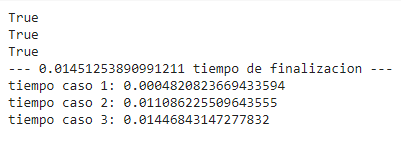
\includegraphics{Algoritmo 1}
    \centering
\end{figure}

\text Resultados del Segundo Algoritmo:

\begin{figure}[H]
	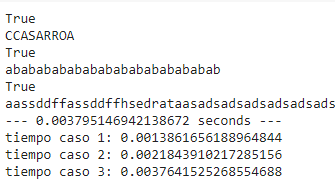
\includegraphics{Algoritmo 2}
    \centering
\end{figure}

\end{document}